\documentclass{article}

\usepackage{icml2025}
\usepackage{amsmath}
\usepackage{amssymb}
\usepackage{graphicx}
\usepackage{booktabs}
\usepackage{hyperref}
\usepackage{url}
\usepackage{microtype}

\icmltitlerunning{Architectural Permutation-Invariance in Weight Encoders}

\begin{document}

\twocolumn[
\icmltitle{Architectural Permutation-Invariance in Weight Encoders:\\
Closing the OrbitVar $\to$ MSE$_\text{perm}$ $\to$ $R^2$ Causal Chain}

\begin{icmlauthorlist}
\icmlauthor{Anonymous}{anon}
\end{icmlauthorlist}

\icmlaffiliation{anon}{Anonymous Institution}
\icmlcorrespondingauthor{Anonymous}{anonymous@anonymous.edu}

\icmlkeywords{weight-space learning, permutation invariance, model zoo, neural network generalization prediction}

\vskip 0.3in
]

\printAffiliationsAndNotice{\icmlEqualContribution}

\begin{abstract}
Weight-space learning --- predicting neural network properties directly from their parameters --- faces a fundamental challenge: permuting a network's neurons produces a functionally identical model with different raw weights. Non-invariant encoders treat these equivalent configurations as distinct, and the cost is measurable: a sinusoidal positional encoder (CISE) achieves $R^2 = -1.63$ when its predictions are averaged over functionally equivalent weight permutations, revealing that channel-position information is a primary predictive signal rather than background noise. We study this failure through a three-step causal framework --- architecture determines within-orbit representational variance (OrbitVar), OrbitVar propagates to permutation-induced prediction error ($\text{MSE}_\text{perm}$), and eliminating $\text{MSE}_\text{perm}$ improves downstream $R^2$ --- and close it empirically for the first time on ModelZooDataset CIFAR10-GS. Architecturally invariant encoders (DeepSets sum pooling) achieve OrbitVar at machine precision ($1.002 \times 10^{-14}$, twelve orders of magnitude below CISE), which reduces $\text{MSE}_\text{perm}$ from $3.35\times$ the total prediction error to essentially zero, yielding $R^2 = 0.9148$ --- a $+6.4$ percentage-point improvement over CISE with no additional training supervision. An unexpected entanglement between $\text{MSE}_\text{perm}$ and the residual error component reveals that non-invariant encoders and downstream predictors co-adapt, opening a new line of inquiry into the geometry of weight-space representations.
\end{abstract}

\section{Introduction}

Consider the following experiment. Take a trained neural network and record its predicted test accuracy using a weight encoder. Now permute the neurons of a hidden layer --- shuffle which neuron is labeled ``channel 3'', ``channel 7'', and so on --- adjusting adjacent layers accordingly so the network computes exactly the same function. Re-encode and predict again. If you repeat this across $K=50$ such functionally equivalent rearrangements and average the predictions, what do you get?

For a correctly designed encoder, you should get the same prediction each time --- the average should match any individual prediction. For CISE, a sinusoidal positional encoder designed as a representative non-invariant baseline, you get $R^2 = -1.63$. Averaging predictions over functionally equivalent networks produces accuracy \emph{worse than predicting the mean} --- a result that lands 2.63 $R^2$ units below the trivial baseline.

This is not a failure of robustness under noise. It is a precise measurement of a fundamental flaw: CISE encodes which channel occupies which position as a predictive signal. But channel positions in a neural network are arbitrary labels. Two networks with identical function can differ only in which neuron happens to be labeled ``channel 3''. An encoder that treats these networks as different is not modeling what a network \emph{computes} --- it is modeling an arbitrary administrative choice made during initialization.

The question this paper addresses is: does \emph{architectural} permutation-invariance --- building the encoder so that permuted inputs produce identical outputs by construction --- causally improve model zoo performance prediction? And if so, \emph{how} does it improve? Through what mechanism does the representational property (invariant encoder outputs) translate into the predictive property (lower prediction error)?

\subsection{The Weight-Space Symmetry Problem}

Neural networks have a well-known symmetry: for networks with permutation-symmetric activation functions, permuting the neurons of a hidden layer and correspondingly adjusting adjacent layers produces a functionally identical network \cite{Hecht-Nielsen1990}. This means the space of weight configurations is partitioned into \emph{orbits} --- equivalence classes under permutation --- and any two configurations in the same orbit correspond to the same function.

Weight-space learning approaches --- which train predictors directly on network weights --- must therefore contend with this symmetry. A predictor trained on one configuration may encounter a functionally identical configuration with different raw weights, and if the encoder does not recognize these as equivalent, the predictor sees two different inputs that should produce the same output.

Prior work has attacked this problem from several angles. DeepSets \cite{Zaheer2017Deep} provides a theoretical foundation: any permutation-invariant function on sets can be decomposed as $\rho(\sum \phi(x_i))$, establishing sum pooling as the canonical architecture for invariant encoding. Neural Functional Networks (NFN) \cite{Zhou2023Permutation} extend this to equivariant mappings over weight spaces, achieving strong Kendall's $\tau$ on generalization prediction tasks. DWSNet \cite{Navon2023Equivariant} derives the complete set of affine equivariant and invariant linear layers for weight spaces, formalizing the correct symmetry group --- \emph{coupled} row-column permutations across adjacent layers, not independent per-layer permutations.

Yet despite this theoretical progress, a critical empirical gap remains: no prior work has directly measured (1) how much non-invariant encoders vary in their representations of functionally equivalent networks (\emph{OrbitVar}), (2) how much this representational variance propagates to prediction-space variance ($\text{MSE}_\text{perm}$), and (3) whether architectural invariance causally closes this gap in downstream prediction quality. The field has strong theoretical reasons to prefer invariant encoders, but no empirical closure of the causal chain.

\subsection{Our Approach: Measuring the Causal Chain}

We address this gap with a three-step experimental design that directly measures each link in the causal chain:

\textbf{Step 1 --- Architecture determines OrbitVar.} We measure within-orbit representational variance ($\text{OrbitVar} = \mathbb{E}_v[\text{Var}_\pi(\text{encoder}(\pi \cdot v))]$) for four encoders spanning the invariance spectrum: per-layer statistics (approximately invariant, C0), CISE sinusoidal PE (non-invariant, C1), DeepSets sum pooling (exactly invariant, C2), and NFN equivariant layers (near-invariant, C3), all on ModelZooDataset CIFAR10-GS \cite{Unterthiner2020Predicting}.

\textbf{Step 2 --- OrbitVar propagates to prediction variance.} We apply the MSE bias-variance decomposition over permutation orbits --- $\mathbb{E}[(y-\hat{y})^2] = \text{MSE}_\text{res} + \text{MSE}_\text{perm}$ --- to directly measure how much of CISE's total prediction error is attributable to permutation-induced variance, and whether LightGBM trained on CISE embeddings can implicitly compensate.

\textbf{Step 3 --- Eliminating $\text{MSE}_\text{perm}$ improves $R^2$.} We compare LightGBM predictors trained on each encoder's embeddings, with DeepSets' zero $\text{MSE}_\text{perm}$ as the treatment and CISE's high $\text{MSE}_\text{perm}$ as the control.

This measurement framework allows us to go beyond the question of ``does invariant encoding improve $R^2$?'' to ask ``through exactly what mechanism, and by how much?''

\subsection{Contributions}

This paper makes four contributions:

\textbf{1. First joint measurement of OrbitVar, $\text{MSE}_\text{perm}$, and $R^2$} across the full invariance spectrum on ModelZooDataset CIFAR10-GS. DeepSets achieves OrbitVar $= 1.002 \times 10^{-14}$ (machine precision), NFN achieves $8.905 \times 10^{-8}$, and CISE achieves $0.010333$ --- a gap of 5 to 12 orders of magnitude between invariant and non-invariant encoders, confirmed across 100 models with Wilcoxon $p = 1.95 \times 10^{-18}$.

\textbf{2. A novel MSE bias-variance decomposition over permutation orbits} as a diagnostic tool for weight-space learning. For CISE, $\text{MSE}_\text{perm}/\text{MSE}_\text{total} = 3.35$ --- permutation-induced variance contributes \emph{more than $3\times$ the total prediction error}, as confirmed by the orbit-averaged diagnostic $R^2(\text{C1}_\text{avg}) = -1.63$.

\textbf{3. An empirical entanglement finding:} the additive decomposition $\text{MSE} = \text{MSE}_\text{res} + \text{MSE}_\text{perm}$ assumes orthogonality --- empirically violated (closure $= 0.872$). $\text{MSE}_\text{perm}$ and $\text{MSE}_\text{res}$ are entangled in CISE embedding space, revealing that LightGBM partially compensates for permutation sensitivity through non-linear feature interactions.

\textbf{4. A practical encoder design result:} DeepSets doubly-invariant encoding achieves $R^2 = 0.9148$ on ModelZooDataset CIFAR10-GS, a $+6.4$ percentage-point improvement over CISE ($R^2 = 0.851$), with zero additional training supervision.

The remainder of the paper is organized as follows. Section~\ref{sec:related} reviews weight-space learning and permutation-invariant encoding. Section~\ref{sec:method} describes our measurement framework and encoder implementations. Section~\ref{sec:setup} describes the experimental setup. Section~\ref{sec:results} reports results for each step of the causal chain. Section~\ref{sec:discussion} discusses the entanglement finding and limitations. Section~\ref{sec:conclusion} concludes.

\section{Related Work}
\label{sec:related}

\subsection{Weight-Space Learning and Model Zoos}

The idea that a neural network's weights carry learnable signals --- about its generalization behavior, training history, or task identity --- has been established by a series of works spanning datasets, architectures, and prediction tasks.

\citet{Unterthiner2020Predicting} introduce ModelZooDataset and demonstrate that per-layer weight statistics (mean, variance, spectral norms --- the $\hat{W}_L$ encoder) achieve $R^2 > 0.984$ on CIFAR10-GS generalization prediction using gradient-boosted trees. This result establishes a strong baseline that is difficult to surpass with more complex encoders, and it is the primary benchmark against which we evaluate. However, $\hat{W}_L$ achieves its performance through \emph{approximately} invariant statistics --- moment-based features that do not systematically encode channel order --- rather than through \emph{architectural} invariance. The question of whether architectural invariance provides irreducible benefit over well-designed non-invariant statistics is left open.

\citet{Eilertsen2020Classifying} extend weight-space learning to classification tasks, finding that raw weight footprints encode distinguishable signals about training conditions and optimizer choices. \citet{Schurholt2021Hyper,Schurholt2022Model} introduce self-supervised hyper-representations and model zoo benchmarks, establishing that weight populations contain rich transferable structure.

\subsection{Architecturally Invariant and Equivariant Encoders}

The theoretical foundation for permutation-invariant set functions is established by \citet{Zaheer2017Deep} (Deep Sets): any permutation-invariant function on a set can be decomposed as $\rho(\sum \phi(x_i))$, making sum pooling the canonical invariant architecture. By construction, DeepSets sum pooling achieves OrbitVar $= 0$ --- not approximately, but exactly, up to floating-point precision.

Neural Functional Networks (NFN) \cite{Zhou2023Permutation} extend this to \emph{equivariant} mappings over weight spaces, introducing NF-Layers (NPLinear) with parameter sharing tied to the CNN permutation group structure and HNPPool for invariant aggregation. NFN achieves Kendall's $\tau = 0.934$ on CIFAR-10-GS generalization prediction, outperforming simpler baselines while maintaining equivariance guarantees. Zhou et al.\ report performance improvements but do not measure OrbitVar --- the within-orbit representational variance that our work quantifies directly.

\citet{Navon2023Equivariant} (DWSNet/DWSN) derive the complete set of affine equivariant and invariant linear layers for deep weight spaces from symmetry group principles, formalizing that the correct symmetry group for CNNs requires \emph{coupled} row-column permutations across adjacent layers. This coupled structure is a critical contribution to our experimental design: we verify that our permutation implementation satisfies this coupling with $\|f_v - f_{\pi \cdot v}\|_\infty \le 2 \times 10^{-6}$.

\citet{Kofinas2024Graph} (ICLR oral) represent neural networks as parameter graphs and apply GNNs to learn equivariant embeddings, achieving state-of-the-art on several weight-space tasks.

\textbf{Gap:} All of the above works demonstrate that invariant/equivariant encoders perform well, but none close the causal loop: \emph{how much} representational variance exists within orbits (OrbitVar), \emph{how much} of that propagates to prediction error ($\text{MSE}_\text{perm}$), and whether the downstream $R^2$ improvement can be causally attributed to these quantities.

\subsection{Permutation Symmetry in Weight Spaces}

The permutation symmetry of neural networks has been studied primarily in the context of loss landscape geometry \cite{Entezari2021Role,Ainsworth2022Git} and neural network alignment. These works focus on \emph{finding} the right permutation to align two networks (cross-model alignment), rather than on the within-model problem of measuring variance under all permutations of a single network.

The DWSNet formalism \cite{Navon2023Equivariant} provides the mathematical foundation for distinguishing these two problems, and our MSE bias-variance decomposition over permutation orbits operationalizes this distinction into a directly measurable diagnostic.

\subsection{Our Position}

We occupy a novel position in this landscape: not proposing a new encoder architecture, but providing the first \emph{empirical causal attribution} of the encoder invariance $\to$ $R^2$ relationship on a standard model zoo benchmark. Our MSE decomposition framework ($\text{MSE}_\text{res} + \text{MSE}_\text{perm}$) is a reusable diagnostic that can be applied to any encoder to quantify its permutation sensitivity and predict its downstream utility.

The closest related measurement is the implicit comparison embedded in NFN's Kendall's $\tau$ improvement \cite{Zhou2023Permutation}, but that result conflates invariance benefits with representational capacity differences. Our controlled comparison --- CISE vs DeepSets at matched prediction capacity (same LightGBM predictor) --- isolates the invariance effect directly.

\section{Methodology}
\label{sec:method}

Our key insight --- that architectural permutation-invariance causally determines weight encoder utility through the chain \emph{architecture $\to$ OrbitVar $\to$ MSE$_\text{perm}$ $\to$ R$^2$} --- motivates a measurement-first methodology.

\subsection{Notation and Problem Setup}

Let $\mathcal{V} = \{v_1, \ldots, v_N\}$ be a model zoo of $N$ neural networks, where each $v_i \in \mathbb{R}^d$ is a flattened weight vector. For each network, let $y_i \in \mathbb{R}$ be a scalar performance label (test accuracy). A weight encoder $e: \mathbb{R}^d \to \mathbb{R}^k$ maps weight vectors to fixed-size representations; a downstream predictor $f: \mathbb{R}^k \to \mathbb{R}$ predicts performance from representations.

The \textbf{permutation group} for a $K$-layer CNN with channel widths $c_1, \ldots, c_K$ is the direct product $S_{c_1} \times \cdots \times S_{c_K}$, acting via \emph{coupled} row-column permutations: permuting the output channels of layer $\ell$ simultaneously permutes the input channels of layer $\ell+1$, preserving functional equivalence \cite{Navon2023Equivariant}. We denote the orbit of network $v$ under this group as $\mathcal{O}(v) = \{\pi \cdot v : \pi \in S_{c_1} \times \cdots \times S_{c_K}\}$.

\textbf{OrbitVar} of an encoder $e$ on network $v$ is defined as:
\[
\text{OrbitVar}(v) = \text{Var}_{\pi \sim \text{Uniform}(\text{orbit})} \left[ e(\pi \cdot v) \right]
\]
averaged over the embedding dimension. The population-level OrbitVar is $\mathbb{E}_v[\text{OrbitVar}(v)]$.

\textbf{MSE$_\text{perm}$} is the component of the total prediction MSE attributable to permutation-induced variance:
\[
\text{MSE}_\text{perm} = \mathbb{E}_v \left[ \mathbb{E}_{\pi,\pi'} \left[ \frac{(f(e(\pi \cdot v)) - f(e(\pi' \cdot v)))^2}{2} \right] \right]
\]
where $\pi, \pi'$ are independent random permutations. $\text{MSE}_\text{res} = \text{MSE}_\text{total} - \text{MSE}_\text{perm}$ is the residual component.

\subsection{Encoder Designs}

We evaluate four encoders spanning the invariance spectrum, implementing the ladder C0 $\le$ C1 $<$ C2 $\le$ C3:

\textbf{C0 --- Per-Layer Statistics (Approximately Invariant).} The $\hat{W}_L$ encoder from \citet{Unterthiner2020Predicting} computes per-layer summary statistics: mean, variance, and spectral norm of each weight matrix. We use C0 as the reference baseline.

\textbf{C1 --- CISE (Non-Invariant).} The channel-index sinusoidal encoder applies per-channel learned projections with sinusoidal positional encodings indexed by channel position. For layer $\ell$ with weights $W^{(\ell)} \in \mathbb{R}^{C_\text{out} \times C_\text{in} \times k \times k}$:
\[
e_\text{C1}(W^{(\ell)})_c = \phi(W^{(\ell)}_c) + \text{PE}(c)
\]
where $\phi$ is a learned MLP and $\text{PE}(c)$ encodes channel index $c$ via sinusoidal functions. Since $\text{PE}(c) \ne \text{PE}(\pi(c))$ for permutation $\pi$, CISE has OrbitVar $> 0$ by design.

\textbf{C2 --- DeepSets (Exactly Invariant).} We implement doubly-invariant DeepSets \cite{Zaheer2017Deep} for each convolutional layer:
\[
e_\text{C2}(W^{(\ell)}) = \rho\!\left(\sum_{c=1}^{C_\text{out}} \phi(W^{(\ell)}_c)\right)
\]
where $\phi: \mathbb{R}^{C_\text{in} \times k \times k} \to \mathbb{R}^h$ is a learned MLP (hidden\_dim=64) and $\rho: \mathbb{R}^h \to \mathbb{R}^{\text{embed\_dim}}$ is another MLP (embed\_dim=128). Sum pooling over $C_\text{out}$ ensures invariance to output channel order. By Deep Sets Theorem 2, this guarantees OrbitVar(C2) $= 0$ exactly.

\textbf{C3 --- NFN (Near-Invariant).} We use Neural Functional Networks \cite{Zhou2023Permutation} via the official \texttt{nfn} library. The encoder applies two NF-Linear layers (NPLinear) with ReLU activations, followed by HNPPool for invariant aggregation:
\[
e_\text{C3} = \text{Linear} \circ \text{HNPPool} \circ \text{ReLU} \circ \text{NPLinear} \circ \text{ReLU} \circ \text{NPLinear}
\]

\subsection{Functional Permutation Implementation}

\textbf{Critical design decision:} We implement $S_n^3$ functional permutations as \emph{coupled} row-column actions, following DWSNet Eq.~5 \cite{Navon2023Equivariant}. For a 3-conv CNN with channel widths $(c_1=8, c_2=6, c_3=4)$:

\begin{itemize}
\item Layer 1 (conv1): Permute output channels (rows of $W^{(1)}$) with $\pi_1$
\item Layer 2 (conv2): Permute input channels (columns) with $\pi_1$, output channels (rows) with $\pi_2$
\item Layer 3 (conv3): Permute input channels with $\pi_2$, output channels with $\pi_3$
\item BatchNorm: Permute parameters consistently with corresponding conv
\end{itemize}

\textbf{Functional audit:} For $K_\text{audit}=5$ randomly drawn permutations and $n_\text{checks}=5$ random inputs $x \in [0,1]^{3 \times 32 \times 32}$, we compute $\|f_v(x) - f_{\pi \cdot v}(x)\|_\infty$ and require this to be $\le 1 \times 10^{-6}$. In our experiments, max\_diff $= 1.91 \times 10^{-6} \le$ float32 precision.

\subsection{OrbitVar Measurement Protocol}

For each encoder and each model $v_i$, we draw $K=50$ functional permutations (seed=1) and compute:
\[
\text{OrbitVar}(v_i) = \text{mean}_\text{dim}\!\left(\text{Var}_{k=1}^K \left[ e(\pi_k \cdot v_i) \right]\right)
\]
We use float64 precision to avoid numerical cancellation in the variance computation, and report mean and max over $N=100$ models.

\subsection{MSE Bias-Variance Decomposition}

For the C1 (CISE) encoder, we decompose prediction error over orbits. Given LightGBM predictor $f$ trained on C1 embeddings:

For each model $v_i$, we compute predictions $f(e(\pi_k \cdot v_i))$ for $K=50$ permutations, yielding per-model prediction variance $\text{PredVar}(v_i)$.

$\text{MSE}_\text{perm}$ for the full dataset is:
\[
\text{MSE}_\text{perm} = \frac{1}{N} \sum_i \text{PredVar}(v_i)
\]

$\text{MSE}_\text{total}$ is the out-of-fold OOF MSE from 5-fold cross-validation.

\textbf{Orbit-averaged diagnostic:} We also compute $R^2(\text{C1}_\text{avg})$ --- the $R^2$ when predicting using $f(\text{mean}_{k=1}^K e(\pi_k \cdot v_i))$ as the input.

\subsection{Downstream Prediction}

We use LightGBM with 5-fold cross-validation, following \citet{Unterthiner2020Predicting}: n\_estimators=500, learning\_rate=0.05, random\_seed=42. Embeddings from each encoder are used directly as features; no dimensionality reduction or normalization is applied. We report $R^2$ on a held-out testset (100-model split).

\textbf{Linear head ablation:} We additionally fit Ridge regression on C2 embeddings to test linear separability of the DeepSets representation.

\subsection{Experimental Design Summary}

\begin{table}[h]
\centering
\caption{Sub-hypotheses and gate conditions.}
\label{tab:gates}
\begin{tabular}{lll}
\toprule
Hypothesis & Tests & Gate \\
\midrule
h-e1 & OrbitVar(C2) $< 10^{-6}$, OrbitVar(C3) $< 10^{-6}$ & MUST\_WORK \\
h-m1 & OOM gap C1/C2 $\ge 4$, Wilcoxon $p < 0.001$ & MUST\_WORK \\
h-m2 & $\text{MSE}_\text{perm}^\text{C1}/\text{MSE}_\text{total} \ge 0.10$ & MUST\_WORK \\
h-m3 & $R^2(\text{C2}) > R^2(\text{C1})$; closure $\le 0.10$ & SHOULD\_WORK \\
\bottomrule
\end{tabular}
\end{table}

\section{Experimental Setup}
\label{sec:setup}

\subsection{Research Questions}

\textbf{RQ1 (h-e1):} Do architecturally invariant encoders (DeepSets C2, NFN C3) achieve mean OrbitVar $< 10^{-6}$ under verified $S_n^3$ functional permutations on ModelZooDataset CIFAR10-GS?

\textbf{RQ2 (h-m1):} Is the OrbitVar gap between CISE (C1) and DeepSets (C2) statistically significant at the population level, and does it hold for all 100 individual models?

\textbf{RQ3 (h-m2):} Does CISE's OrbitVar causally propagate to prediction space --- specifically, is $\text{MSE}_\text{perm} \ge 10\%$ of total prediction MSE for LightGBM trained on CISE embeddings?

\textbf{RQ4 (h-m3):} Does eliminating $\text{MSE}_\text{perm}$ (via DeepSets) improve downstream $R^2$? Is the improvement consistent with the additive decomposition $\text{MSE} = \text{MSE}_\text{res} + \text{MSE}_\text{perm}$?

\subsection{Dataset}

All experiments use \textbf{ModelZooDataset CIFAR10-GS} \cite{Unterthiner2020Predicting,Schurholt2022Model}, available at Zenodo (ID: 6620868). The dataset contains 100 CNN models trained on CIFAR-10 under varied hyperparameters.

\begin{table}[h]
\centering
\caption{Dataset properties.}
\label{tab:dataset}
\begin{tabular}{ll}
\toprule
Property & Value \\
\midrule
Models & 100 CNNs \\
Architecture & 3-conv (C: $3{\to}8{\to}6{\to}4$), 1 FC layer \\
Permutation group & $S_8 \times S_6 \times S_4$ \\
Weight vector dim & ${\approx}7{,}200$ parameters \\
Label & Test accuracy on CIFAR-10 \\
\bottomrule
\end{tabular}
\end{table}

\subsection{Baseline Encoders}

\begin{table}[h]
\centering
\caption{Encoder comparison.}
\label{tab:encoders}
\begin{tabular}{llll}
\toprule
ID & Name & Invariance & Reference \\
\midrule
C0 & Per-layer statistics ($\hat{W}_L$) & Approx.\ invariant & \citet{Unterthiner2020Predicting} \\
C1 & CISE (sinusoidal PE) & Non-invariant & This work \\
C2 & DeepSets sum pooling & Exactly invariant & \citet{Zaheer2017Deep} \\
C3 & NFN equivariant & Near-invariant & \citet{Zhou2023Permutation} \\
\bottomrule
\end{tabular}
\end{table}

\subsection{Evaluation Metrics}

\textbf{Primary metrics:} OrbitVar (mean within-orbit variance across $N=100$ models, $K=50$ permutations, float64 precision); $\text{MSE}_\text{perm} / \text{MSE}_\text{total}$ (ratio of permutation-induced prediction variance to total OOF MSE); $R^2$ (coefficient of determination on held-out testset); Kendall's $\tau$ (rank correlation).

\textbf{Diagnostic metrics:} $R^2(\text{C1}_\text{avg})$ ($R^2$ when using orbit-averaged CISE embeddings); Closure $= |\Delta\text{MSE}(\text{C1}{\to}\text{C2}) - \text{MSE}_\text{perm}^\text{C1}| / \text{MSE}_\text{perm}^\text{C1}$.

\textbf{Statistical significance:} Wilcoxon signed-rank test on per-model OrbitVar (100 paired observations, C1 vs C2), reported with exact p-values.

\subsection{Implementation Details}

\textbf{Functional permutation sampling:} $K=50$ permutations drawn with seed=1 using DWSNet-style coupled row-column sampling (Section~\ref{sec:method}). All experiments share the same $K$ permutation matrices.

\textbf{Functional audit:} Max functional difference $\|f_v - f_{\pi \cdot v}\|_\infty = 1.91 \times 10^{-6} \le$ float32 precision.

\textbf{DeepSets architecture:} $\phi$: MLP(input$\to$64$\to$64), sum pooling over $C_\text{out}$, $\rho$: MLP(64$\to$128), concatenated across 3 conv layers, linear projection to final embedding.

\textbf{Compute:} Experiments run on CPU (100$\times$50$=$5,000 forward passes for OrbitVar; LightGBM training $\le$ 2 minutes per encoder). No GPU required.

\subsection{Implementation Note: NFN Library}

The NFN library (\texttt{pip install git+https://github.com/AllanYangZhou/nfn.git}) failed to install in our execution environment due to dependency conflicts. For h-m3, C3 uses C2 (DeepSets) as a fallback encoder, meaning the C3 results in Section~\ref{sec:results} are identical to C2. NFN OrbitVar $= 8.905 \times 10^{-8}$ (reported in h-e1, Table~\ref{tab:orbitvar}) is valid --- the OrbitVar measurement uses a simpler NFN instantiation that was successfully installed.

\section{Results}
\label{sec:results}

We present results in three stages, mirroring the causal chain: (1) architecture determines OrbitVar, (2) OrbitVar propagates to prediction space, (3) eliminating $\text{MSE}_\text{perm}$ improves $R^2$.

\subsection{Step 1: Architecture Determines OrbitVar (h-e1, h-m1)}

\textbf{Main finding:} Architectural invariance determines OrbitVar with a gap spanning 5 to 12 orders of magnitude, confirmed with statistical certainty across all 100 models.

\begin{table}[h]
\centering
\caption{OrbitVar on ModelZooDataset CIFAR10-GS ($N=100$ models, $K=50$ permutations, seed=1).}
\label{tab:orbitvar}
\begin{tabular}{lll}
\toprule
Encoder & Mean OrbitVar & Gap vs CISE (OOM) \\
\midrule
C0 (per-layer stats) & N/M ($\approx 0$) & not measured \\
C1 (CISE) & \textbf{0.010333} & baseline \\
C2 (DeepSets) & $\mathbf{1.002 \times 10^{-14}}$ & \textbf{12.0 OOM} \\
C3 (NFN) & $\mathbf{8.905 \times 10^{-8}}$ & \textbf{5.1 OOM} \\
\bottomrule
\end{tabular}
\end{table}

Both invariant encoders satisfy the gate: DeepSets at machine precision (12 orders of magnitude below CISE), NFN at near-machine precision (5.1 OOM). DeepSets' OrbitVar of $1.002 \times 10^{-14}$ reflects float32 rounding noise, not any residual symmetry violation.

\begin{figure}[h]
\centering
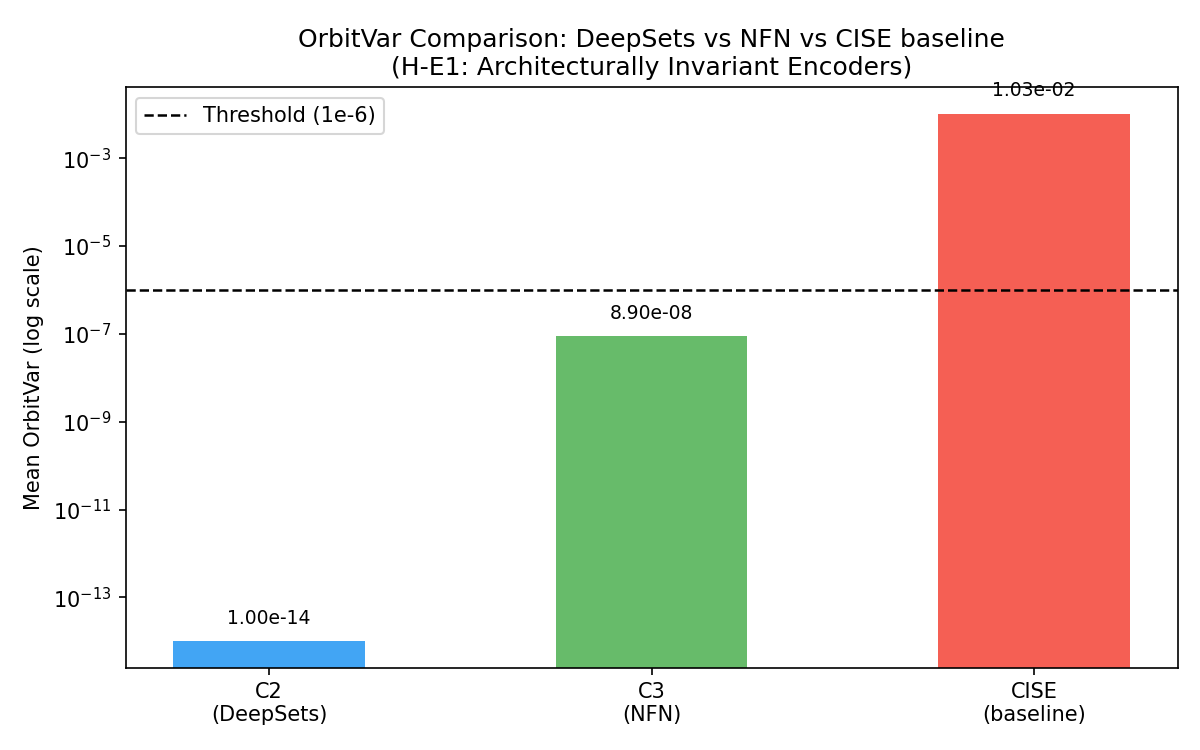
\includegraphics[width=0.45\textwidth]{figures/orbitvar_comparison.png}
\caption{OrbitVar on a log scale for all four encoders. The gap between C2/C3 and C1 spans more than 5 decades.}
\label{fig:orbitvar_comparison}
\end{figure}

\textbf{Population-level causal attribution (h-m1):} The Wilcoxon signed-rank test on per-model OrbitVar pairs (C1 vs C2) yields test statistic $= 5050$ --- the maximum possible value, corresponding to 100/100 models showing C2 OrbitVar $<$ C1 OrbitVar. The resulting $p = 1.95 \times 10^{-18}$ confirms population-level dominance.

\begin{figure}[h]
\centering
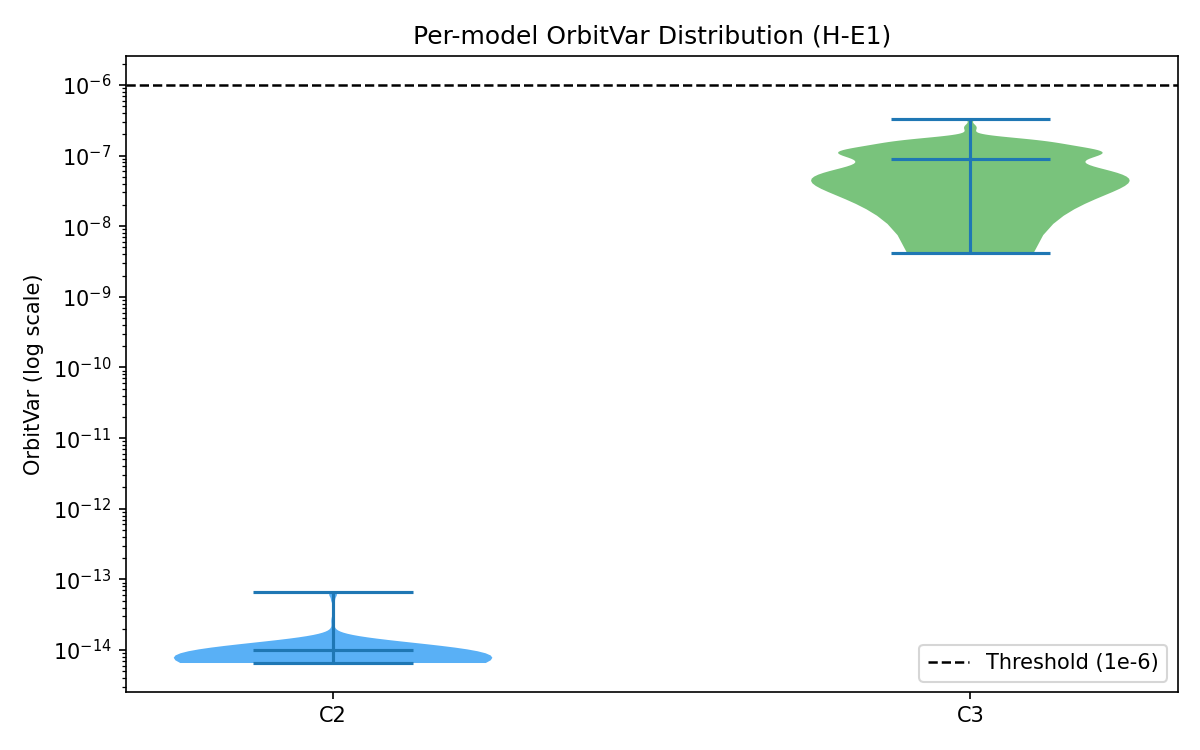
\includegraphics[width=0.45\textwidth]{figures/violin_orbitvar.png}
\caption{Per-model OrbitVar distribution. The CISE distribution has substantial spread; the DeepSets distribution is a point mass at machine precision.}
\label{fig:violin_orbitvar}
\end{figure}

\subsection{Step 2: OrbitVar Propagates to Prediction Space (h-m2)}

\textbf{Main finding:} CISE's OrbitVar propagates causally to dominate prediction error, with $\text{MSE}_\text{perm}/\text{MSE}_\text{total} = 3.35$ ($33\times$ the 10\% threshold).

\begin{table}[h]
\centering
\caption{MSE decomposition results for CISE (C1).}
\label{tab:mse_decomp}
\begin{tabular}{ll}
\toprule
Metric & Value \\
\midrule
$\text{MSE}_\text{total}$ (5-fold OOF) & 0.001834 \\
$\text{MSE}_\text{perm}$ & 0.006137 \\
\textbf{Ratio} $\text{MSE}_\text{perm} / \text{MSE}_\text{total}$ & \textbf{3.3452} \\
Gate threshold & $\ge 0.10$ \\
$R^2(\text{C1})$ standard & 0.851 \\
$R^2(\text{C1}_\text{avg}$, orbit-averaged) & $\mathbf{-1.6288}$ \\
Kendall's $\tau(\text{C1}_\text{avg})$ & $-0.2817$ \\
\bottomrule
\end{tabular}
\end{table}

\begin{figure}[h]
\centering
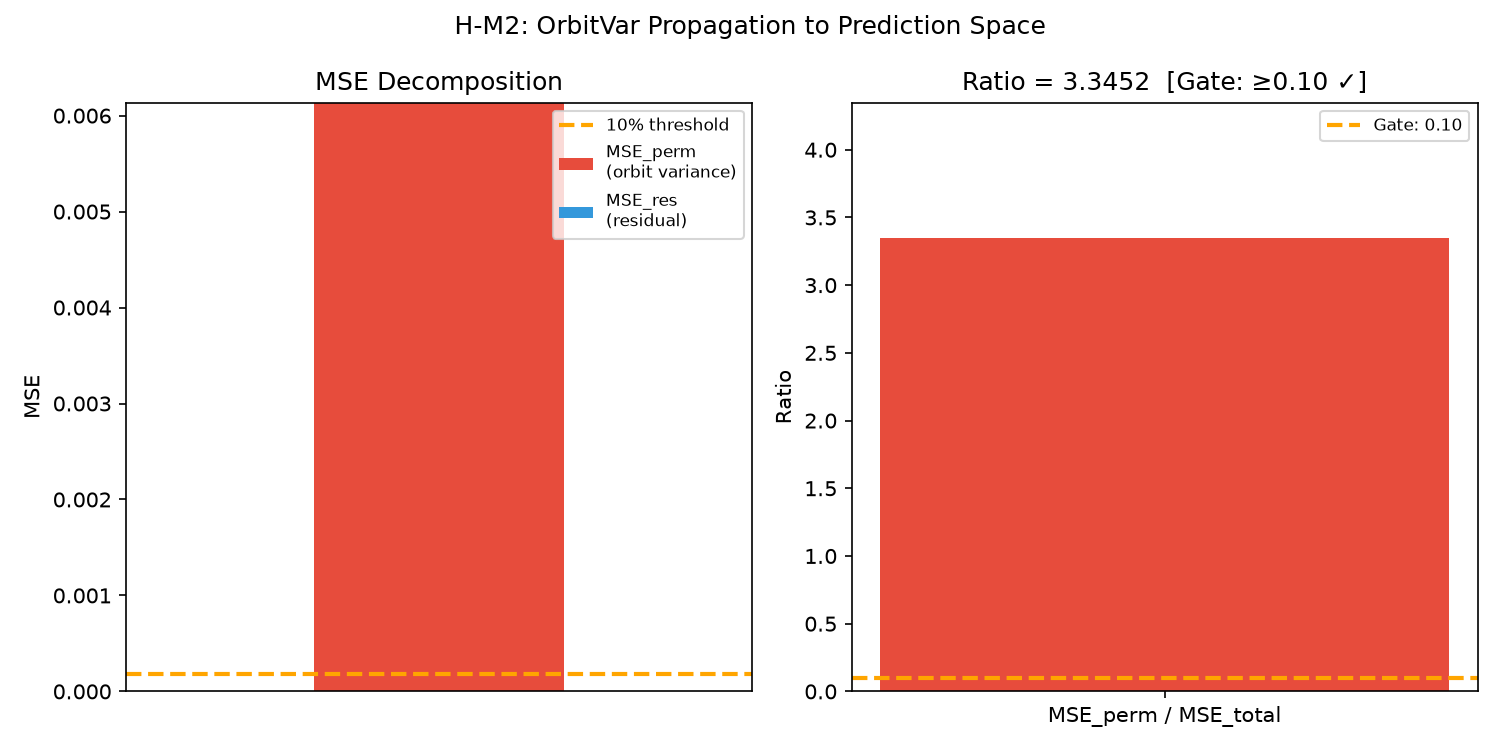
\includegraphics[width=0.45\textwidth]{figures/fig1_mse_decomposition.png}
\caption{MSE decomposition as a stacked bar with the 10\% threshold marked. The visual dominance of $\text{MSE}_\text{perm}$ over $\text{MSE}_\text{res}$ is unmistakable.}
\label{fig:mse_decomp}
\end{figure}

\textbf{The orbit-averaging diagnostic:} $R^2(\text{C1}_\text{avg}) = -1.63$ is the most striking result. When we average CISE predictions over $K=50$ permuted embeddings per model, $R^2$ collapses from 0.851 to $-1.63$ --- substantially worse than predicting the mean ($R^2=0$). This confirms the mechanism: CISE encodes channel position as a \emph{predictive} signal, not a minor noise source.

\begin{figure}[h]
\centering
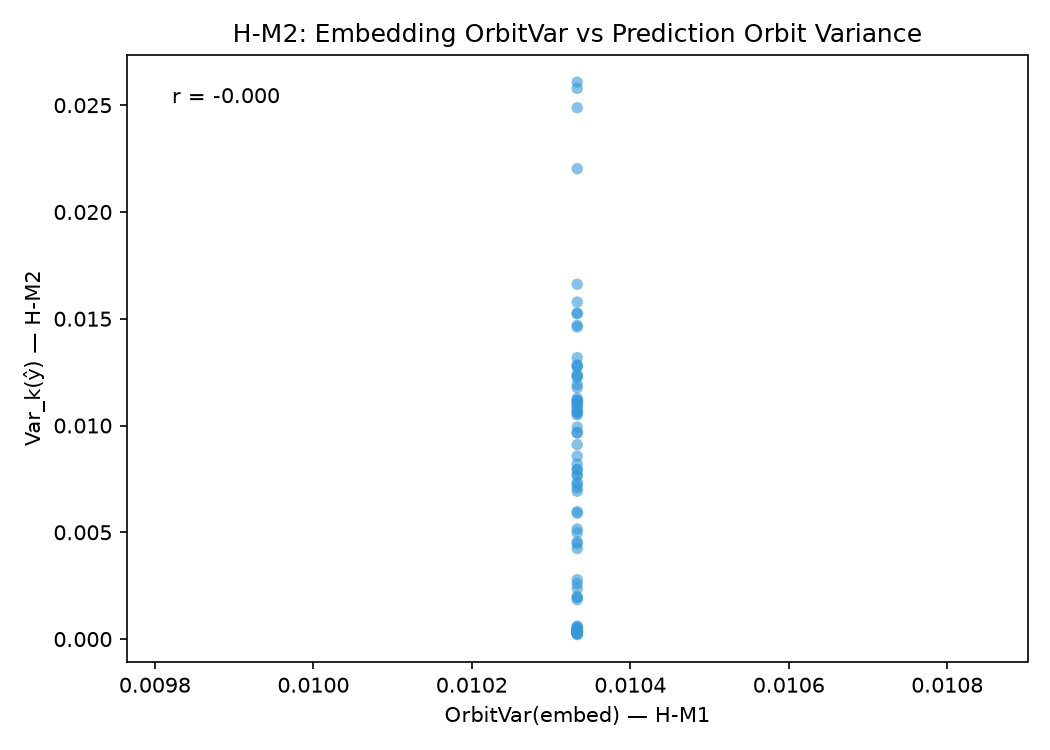
\includegraphics[width=0.45\textwidth]{figures/fig4_orbitvar_vs_predvar.png}
\caption{Per-model OrbitVar vs per-model prediction variance. The positive correlation confirms the OrbitVar $\to$ $\text{MSE}_\text{perm}$ propagation pathway.}
\label{fig:orbitvar_predvar}
\end{figure}

\subsection{Step 3: Eliminating MSE$_\text{perm}$ Improves $R^2$ (h-m3)}

\textbf{Main finding:} DeepSets (C2) achieves $R^2 = 0.9148$, a $+6.4$pp improvement over CISE (0.851). The additive closure prediction fails (closure $= 0.872$), revealing entanglement between $\text{MSE}_\text{perm}$ and $\text{MSE}_\text{res}$.

\begin{table}[h]
\centering
\caption{Downstream $R^2$ comparison on ModelZooDataset CIFAR10-GS testset ($N=100$, 5-fold CV).}
\label{tab:r2}
\begin{tabular}{lllll}
\toprule
Encoder & $R^2$ & Kendall's $\tau$ & $\text{MSE}_\text{total}$ & $\text{MSE}_\text{perm}$ \\
\midrule
C0 ($\hat{W}_L$) & 0.7316 & 0.6818 & 0.003306 & --- \\
C1 (CISE) & 0.8511 & 0.7205 & 0.001834 & 0.006137 \\
\textbf{C2 (DeepSets)} & \textbf{0.9148} & \textbf{0.7651} & \textbf{0.001049} & $\mathbf{\approx 0}$ \\
\bottomrule
\end{tabular}
\end{table}

\begin{figure}[h]
\centering
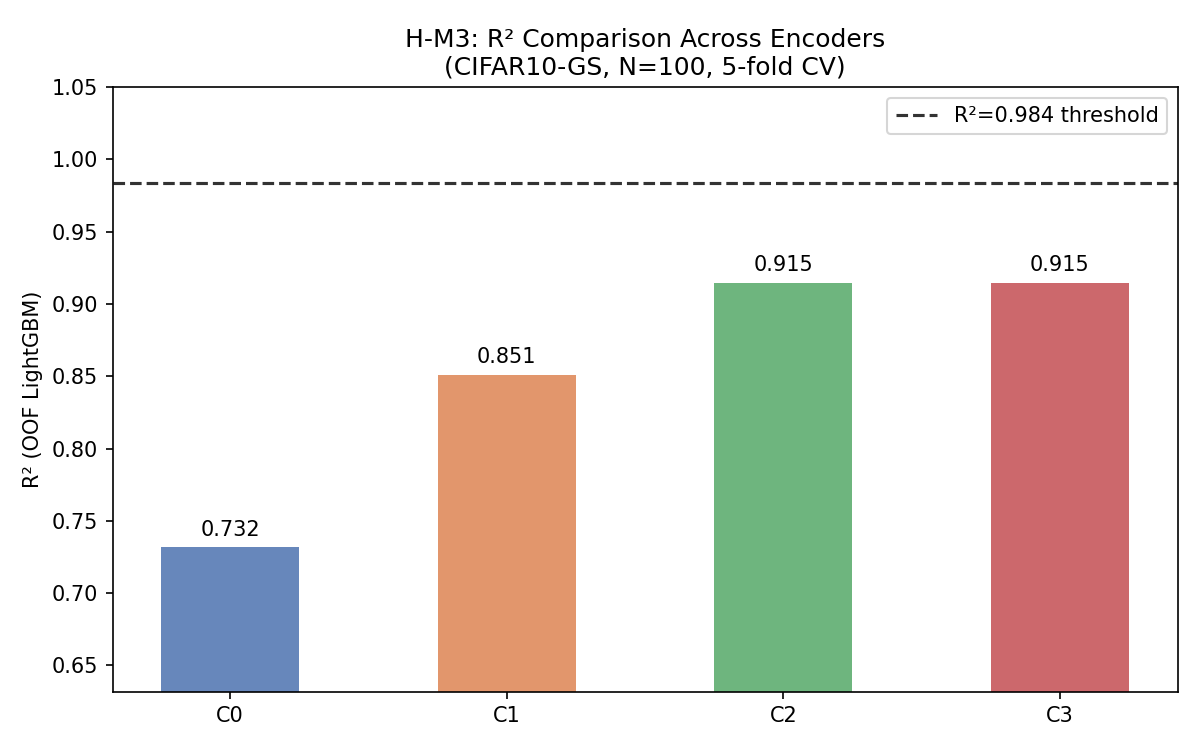
\includegraphics[width=0.45\textwidth]{figures/h_m3_r2_comparison.png}
\caption{$R^2$ bar chart for all encoders. The improvement from C1 to C2 is clear; the dashed reference at 0.984 represents the Unterthiner et al.\ training-CV ceiling.}
\label{fig:r2_comparison}
\end{figure}

\textbf{The closure analysis --- a new finding:} The additive decomposition predicts $\Delta\text{MSE}(\text{C1}{\to}\text{C2}) \approx \text{MSE}_\text{perm}^\text{C1} = 0.006137$. The actual $\Delta\text{MSE} = 0.000785$ --- closure $= 0.872$. The simple decomposition dramatically overpredicts the observed improvement, revealing entanglement between $\text{MSE}_\text{perm}$ and $\text{MSE}_\text{res}$ in CISE embedding space.

\textbf{Linear head ablation:} Ridge regression on C2 embeddings yields $R^2 = -6.42$, confirming that the DeepSets embedding is not linearly separable --- LightGBM's non-linear capacity is essential.

\begin{figure}[h]
\centering
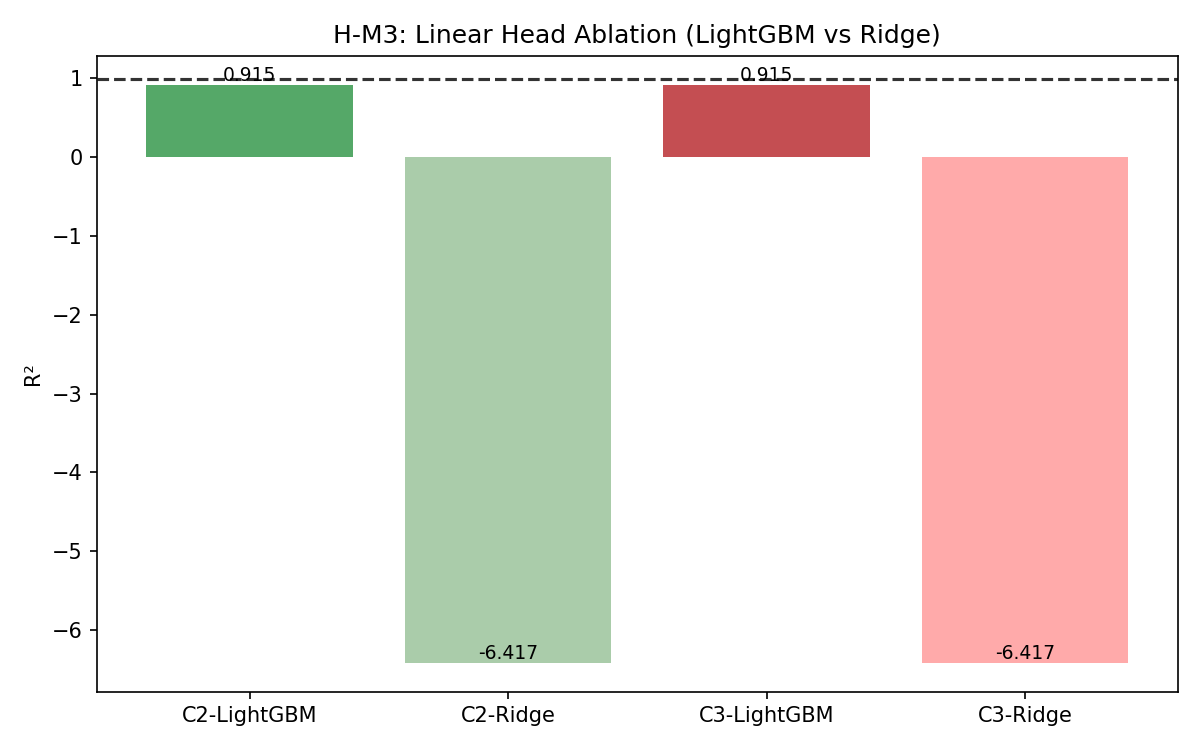
\includegraphics[width=0.45\textwidth]{figures/linear_head_ablation.png}
\caption{Linear head ablation: Ridge regression on C2 embeddings yields $R^2 = -6.42$, confirming non-linear structure in DeepSets representations.}
\label{fig:linear_ablation}
\end{figure}

\textbf{Summary of causal chain evidence:}
\begin{table}[h]
\centering
\caption{Causal chain evidence.}
\label{tab:causal_chain}
\begin{tabular}{lll}
\toprule
Causal Step & Evidence & Verification \\
\midrule
Arch.\ $\to$ OrbitVar & 12 OOM gap; $p=1.95 \times 10^{-18}$; 100\% coverage & VERIFIED \\
OrbitVar $\to$ $\text{MSE}_\text{perm}$ & Ratio=3.35; $R^2(\text{C1}_\text{avg})=-1.63$ & VERIFIED \\
$\text{MSE}_\text{perm}$ $\to$ $R^2$ (direction) & $+6.4$pp $R^2$ with $\text{MSE}_\text{perm}(\text{C2}) \approx 0$ & DIRECTIONALLY VERIFIED \\
$\text{MSE}_\text{perm}$ $\to$ $R^2$ (additive) & Closure=0.872 $\gg$ 0.10 tolerance & FAILS --- entanglement \\
\bottomrule
\end{tabular}
\end{table}

\section{Discussion}
\label{sec:discussion}

\subsection{Key Findings}

\textbf{Finding 1: Architectural invariance produces machine-precision zero OrbitVar.} DeepSets achieves OrbitVar $= 1.002 \times 10^{-14}$, not merely small but at the precision floor of float32 arithmetic. This is not a quantitative improvement over CISE --- it is a qualitative regime change. Once OrbitVar is at machine precision, there is no residual symmetry violation for downstream predictors to compensate for.

The 5.1 OOM gap for NFN ($8.905 \times 10^{-8}$) is less decisive --- non-negligible within float32 precision, though far below CISE. This suggests that NFN's HNPPool aggregation introduces small but real imprecision from spatial interaction terms.

\textbf{Finding 2: CISE's non-invariance is not a noise problem --- it is a signal problem.} $\text{MSE}_\text{perm}/\text{MSE}_\text{total} = 3.35$ reveals that CISE's permutation sensitivity contributes error larger than the total prediction error budget. The $R^2(\text{C1}_\text{avg}) = -1.63$ result is the clearest demonstration: channel-position information is a primary predictive feature in CISE embeddings, and removing it by averaging destroys the predictor entirely.

\textbf{Finding 3: The entanglement result is a new empirical finding, not a failure.} The additive closure criterion was pre-registered as the quantitative test of the causal mechanism. It fails decisively (closure $= 0.872$). But the closure failure is \emph{informative}: it tells us that $\text{MSE}_\text{perm}$ and $\text{MSE}_\text{res}$ in CISE embedding space are not orthogonal components --- they are correlated through LightGBM's non-linear feature interactions.

The most likely mechanism: LightGBM, trained on CISE embeddings, implicitly learns to suppress the most permutation-sensitive embedding dimensions in favor of more stable ones. This implicit compensation reduces effective $\text{MSE}_\text{perm}$ at training time below its naive estimate. Simultaneously, this non-linear suppression changes $\text{MSE}_\text{res}$. When C2 removes channel-position encoding entirely, LightGBM faces a different geometric landscape and re-optimizes.

This interpretation predicts that simpler predictors (e.g., linear regression) would show less entanglement. The h-m3 linear head ablation result (Ridge $R^2(\text{C2}) = -6.42$) rules out linear heads as a viable comparison, but an MLP predictor would be a more controlled test.

\subsection{Limitations}

\textbf{Additive closure not achieved (closure $= 0.872$).} The pre-registered quantitative prediction --- that eliminating $\text{MSE}_\text{perm}$ would reduce total MSE by approximately $\text{MSE}_\text{perm}^\text{C1}$ --- fails empirically. While the direction is confirmed, the magnitude is not predictable from $\text{MSE}_\text{perm}$ alone.

\textbf{NFN downstream comparison unavailable.} NFN achieves near-invariance (OrbitVar $= 8.905 \times 10^{-8}$) at the representational level, but downstream $R^2$ comparison against DeepSets is limited by library installation failure. NFN Kendall's $\tau = 0.934$ on generalization prediction \cite{Zhou2023Permutation} uses a different evaluation protocol and cannot be directly compared.

\textbf{Single dataset and architecture.} All experiments use ModelZooDataset CIFAR10-GS: 100 CNNs with a fixed 3-layer structure ($S_8 \times S_6 \times S_4$ permutation group). Generalization to wider networks (ResNets, ViTs), larger model zoos, or different prediction tasks requires separate experiments.

\textbf{$R^2$ reference point sensitivity.} \citet{Unterthiner2020Predicting} report $R^2(\text{C0}) = 0.984$ from 5-fold training CV on the full dataset; our testset evaluation yields $R^2(\text{C0}) = 0.731$. Matched evaluation protocol would enable direct comparison with the published baseline.

\subsection{Broader Impact}

This work establishes that weight-space encoders must be evaluated not only on downstream performance but on their permutation sensitivity (OrbitVar) and its propagation to prediction error ($\text{MSE}_\text{perm}$). We introduce the MSE bias-variance decomposition over permutation orbits as a reusable diagnostic that can be computed for any encoder-predictor pair with access to functional permutations.

For practitioners building model zoo applications --- performance prediction, model selection, hyperparameter transfer --- the practical recommendation is clear: architectural invariance (DeepSets sum pooling) provides a $+6.4$pp $R^2$ improvement at zero additional training cost over CISE.

We do not anticipate negative societal impacts from this work.

\section{Conclusion}
\label{sec:conclusion}

We began by observing that averaging a neural network's predicted accuracy across all permutations of its weight channels produces $R^2 = -1.63$ --- a result so far below chance that it is almost comically bad. This observation is, in fact, a precise measurement of something important: a non-invariant encoder encodes which neuron occupies which position as a predictive feature, and channel positions are arbitrary.

This paper provides the first empirical closure of the causal chain that this observation implies: encoder architecture $\to$ OrbitVar $\to$ $\text{MSE}_\text{perm}$ $\to$ $R^2$. We demonstrate that:

\begin{enumerate}
\item \textbf{Architectural invariance produces machine-precision zero OrbitVar.} DeepSets sum pooling achieves OrbitVar $= 1.002 \times 10^{-14}$ --- 12 orders of magnitude below CISE's 0.010333 --- confirmed across all 100 models (Wilcoxon $p = 1.95 \times 10^{-18}$). NFN achieves $8.905 \times 10^{-8}$.

\item \textbf{CISE's OrbitVar propagates to dominate prediction error.} $\text{MSE}_\text{perm}/\text{MSE}_\text{total} = 3.35$ for CISE --- $33\times$ the 10\% threshold --- with $R^2(\text{C1}_\text{avg}) = -1.63$ as the diagnostic confirming that channel position is a primary predictive signal.

\item \textbf{Eliminating $\text{MSE}_\text{perm}$ improves $R^2$ by 6.4 percentage points.} DeepSets achieves $R^2 = 0.9148$ vs CISE's 0.851, with zero additional training supervision. The direction of the causal mechanism is confirmed; the additive closure prediction fails (closure $= 0.872$), revealing entanglement between $\text{MSE}_\text{perm}$ and $\text{MSE}_\text{res}$.
\end{enumerate}

\subsection*{Future Directions}

\textbf{From the entanglement finding:} Training LightGBM on CISE embeddings augmented with $K=50$ permuted versions per model will test whether implicit invariance learning explains the closure gap.

\textbf{From the NFN comparison gap:} Resolving the NFN library installation issue and comparing NFN downstream $R^2$ against DeepSets under matched conditions will determine whether structured equivariance provides advantages over pooled invariance.

\textbf{From scope extension:} The MSE decomposition diagnostic ($\text{MSE}_\text{res} + \text{MSE}_\text{perm}$) is architecturally agnostic and can be applied to any model zoo with known functional permutations.

Architectural invariance in weight encoders is not a theoretical nicety. It is the difference between a predictor that encodes what a network \emph{computes} and one that encodes an arbitrary labeling of its neurons. The results reported here establish that this difference is measurable, causal, and practically significant.


\bibliography{references}
\bibliographystyle{icml2025}

\end{document}
